\documentclass[a4paper]{article}

\usepackage{amsmath}
\usepackage{hyperref}
\usepackage{biblatex}
\usepackage{enumerate}
\usepackage{graphicx}
\usepackage{stmaryrd}
\usepackage[dvipsnames]{xcolor}
\usepackage{listings}
\usepackage{float}
\addbibresource{refs.bib}

\begin{document}

\author{
  Sebastian Miles \\
  \href{mailto:miless@chalmers.se}{miless@chalmers.se}
  \and
  Olle Lapidus \\
  \href{mailto:ollelap@chalmers.se}{ollelap@chalmers.se}
}
\title{DAT565/DIT407 Assignment 2}
\date{2024-09-12}

\maketitle
The goal of this assignment is to practice data cleaning by extracting data from a source that that is not in the format we want. 
Then, we produce plots using the extracted data. The code for generating the .cvs file containing the extracted data can be found in the section \textbf{Extraction Code}. And the code for generating the plots is located in the section \textbf{Plot Code}.\\\\
After extraction, we analyze the closing prices in 2022 by calculating the five-number summary. The summary is shown in Table \ref{tab}. Next, we plot the histogram of the closing prices in 2022. The number of bins was manually chosen as $N=25$ so that the bins would not contain any gaps and are not overly grouped. Thus, $N=25$ was considered an appropriate number of bins.\\\\
When analyzing Figure \ref{scatter}, we can clearly see a general trend: the larger the living area, the higher the closing price. Although there are some deviations, the majority of listings follow this trend. This makes sense intuitively, as a larger area typically results in a higher cost. In Figure \ref{scatter2}, we observe that as the living area increases, the number of rooms also increases.

\begin{table}[h!]
\centering

\begin{tabular}{|c|c|}
\hline
Minimum & 1,650,000 \\
First Quartile (25\%) & 4,012,500 \\
Median (50\%) & 5,000,000 \\
Third Quartile (75\%) & 5,795,000 \\
Maximum & 10,500,000 \\
\hline
\end{tabular}
\caption{Five-Number Summary of Closing Prices in 2022 (in SEK)}
\label{tab}
\end{table}

\begin{figure}[H]
  \begin{center}
    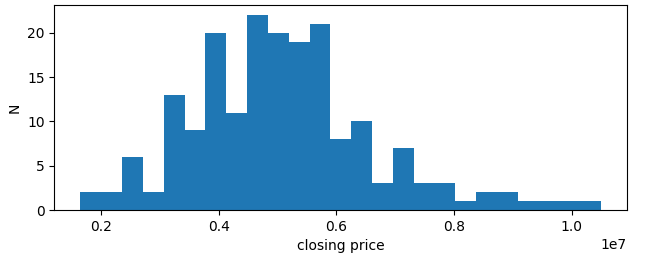
\includegraphics[scale=0.5]{hist.png}
    \caption{Histogram showing the closing prices of houses in 2022.}
    \label{hist}
  \end{center}
\end{figure}

\begin{figure}[H]
  \begin{center}
    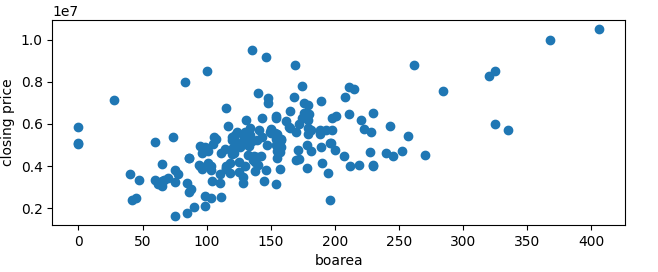
\includegraphics[scale=0.5]{scatter.png}
    \caption{Scatter plot over the closing prices of 2022 in Kungälv.}
    \label{scatter}
  \end{center}
\end{figure}

\begin{figure}[H]
  \begin{center}
    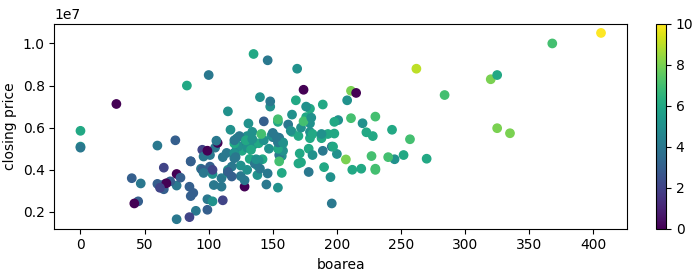
\includegraphics[scale=0.5]{scatter2.png}
    \caption{Scatter plot over closing prices including the number of rooms during 2022 in Kungälv.}
    \label{scatter2}
  \end{center}
\end{figure}

\printbibliography
\appendix

\section*{Extraction code}
\label{app:excode}

\lstset{
	language=Python,
	basicstyle=\ttfamily,
	commentstyle=\color{OliveGreen},
	keywordstyle=\bfseries\color{Magenta},
	stringstyle=\color{YellowOrange},
	numbers=left,
	frame=tblr,
	breaklines=true,
	postbreak=\mbox{\textcolor{red}{$\hookrightarrow$}\space},
}
\begin{lstlisting}
from bs4 import BeautifulSoup
import re

import datetime
import pandas as pd
import os

def ParseDate(date):
    monthDict = {
        'januari' : 1,
        'februari': 2,
        'mars': 3,
        'april': 4,
        'maj': 5,
        'juni': 6,
        'juli': 7,
        'augusti': 8,
        'september': 9,
        'oktober': 10,
        'november': 11,
        'december': 12
    }
    parts = date.split(" ")

    return datetime.datetime(day=int(parts[1]), month=monthDict[parts[2]], year=int(parts[3]))

def Process(html_doc):
    soup = BeautifulSoup(html_doc, 'html.parser')

    cols = 7
    data = [[]*cols for i in range(cols)]
    for listing in soup.find_all ('li', class_ ='sold-results__normal-hit'):
        data[0].append(ParseDate(listing.find('span', class_ ='hcl-label--sold-at').text.strip()))
        data[1].append(listing.find('h2', class_='sold-property-listing__heading').text.strip())
        # Get raw location
        location = listing.select('div.sold-property-listing__location>div')[0].text.strip()
        location = re.sub(r'VillaVilla\s+|\n|  ', '', location) # Remove garbage
        data[2].append(location)

        area = listing.select('div.sold-property-listing__area')[0].text.strip()
        text = re.sub(r'\s+', '', area).split('^2')
        rooms = re.sub(r'rum', '', text[len(text)-1])
        area = 0
        for i in range(len(text)-1):
            for temp in text[i].split('+'):
                area += float(re.sub(',+', '.', re.sub('m+|m^2+', '', temp)))

        data[3].append(area)
        data[4].append(rooms)
        
        if(listing.find('div', class_ ='sold-property-listing__land-area')):
            landarea = listing.select('div.sold-property-listing__land-area')[0].text.strip()
            landarea = re.sub(r'm^2 tomt|\s+', '', landarea) # Remove garbage
            data[5].append(landarea)
        else:
            data[5].append(0) # Land area doesnt exist, maybe an apartment?

        price = re.sub(r'\s+|Slutpris|kr', '', listing.find('span', 'hcl-text').text.strip())
        data[6].append(price)

    df = pd.DataFrame({
        'date': data[0],
        'address': data[1],
        'location': data[2],
        'boarea': data[3],
        'rooms': data[4],
        'landarea': data[5],
        'closing price': data[6],
    })
    return df

folder_path = 'kungalv_slutpriser'
files = os.listdir (folder_path)

table = list()

# For each filename
for file_name in files:
    file_path = os.path.join(folder_path, file_name)
    f = open(file_path, 'r', encoding='utf-8')
    table.append(Process(f.read()))

df = pd.concat(table)

df.to_csv('listings.csv', index = None)

\end{lstlisting}

\section*{Plot code}

\begin{lstlisting}
import pandas as pd
import matplotlib.pyplot as plt
import numpy as np

# Read from file
df = pd.read_csv('listings.csv')

df2 = (df[df['date'].str.contains('2022')])

print(df2['closing price'].describe().loc[['min','25%','50%','75%','max']])

fig, axs = plt.subplots(3, constrained_layout = True , figsize = (7 ,8))

rooms = np.nan_to_num(np.array(pd.to_numeric(df2['rooms'])))
axs [0].hist (df2['closing price'], bins = 25)
sp = axs[2].scatter(df2['boarea'], df2['closing price'], c = rooms , cmap = "viridis")

axs[0].set_xlabel("closing price")
axs[0].set_ylabel("N")
axs[1].scatter(df2['boarea'], df2['closing price'])
axs[1].set_xlabel("boarea")
axs[1].set_ylabel("Closing price")
axs[2].set_xlabel("boarea")
axs[2].set_ylabel("Closing price")

fig.colorbar(sp)
plt.show()
\end{lstlisting}

\end{document}
